\documentclass[12pt]{report} 

\usepackage{palatino}
\usepackage{epsfig}
\usepackage[margin=0.8in]{geometry}

\usepackage{amsmath}
\usepackage{tikz}
\usetikzlibrary{patterns,arrows}

\pagestyle{empty} %%% this results in no pagenumbers (footer is empty}

\setlength{\parindent}{0in}
\setlength{\parskip}{0.05in}

\baselineskip=20pt

\newcommand{\dsps}{\displaystyle}
\newcommand{\pp}{\par \noindent}
\newcommand{\newp}{\vfil \eject}

\begin{document}
\noindent
\vfil \noindent

% Axes

\begin{center}
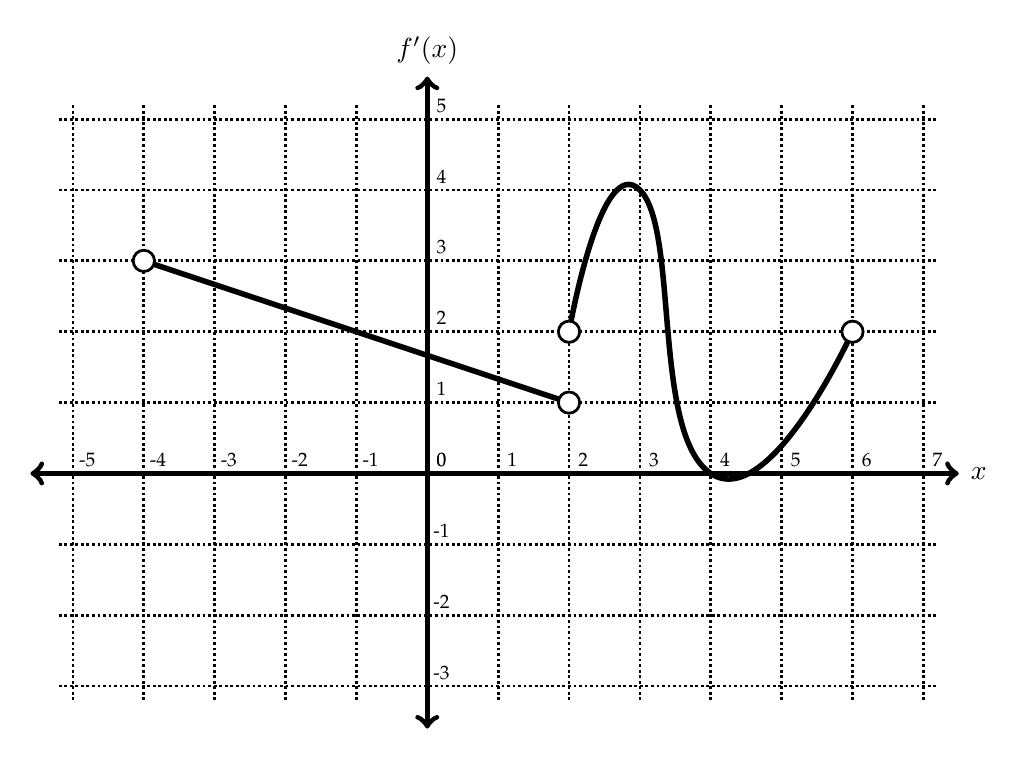
\begin{tikzpicture}[auto,scale=.9, line width=2pt]

\draw [line width=1pt,densely dotted] (-5.2,-3.2) grid (7.2,5.2);
\foreach \x in {-5,-4,...,7} \draw (\x+.2,.19) node {\scriptsize \x};
\foreach \y in {-3,-2,...,5} \draw (.2,\y+.19) node {\scriptsize \y};
\draw [<->] (-5.6,0) -- (7.5,0) node[right] {$x$};
\draw [<->] (0,-3.6) -- (0,5.6) node[above] {$f'(x)$};

\draw plot[smooth, tension=1] coordinates{(2,2) (3,4) (4,0) (6,2)};
\draw (-4,3) -- (2,1);

\draw[line width=1 pt, fill=white] (-4,3) circle (.15);
\draw[line width=1 pt, fill=white] (2,1) circle (.15);
\draw[line width=1 pt, fill=white] (2,2) circle (.15);
\draw[line width=1 pt, fill=white] (6,2) circle (.15);
\end{tikzpicture}
\end{center}

%Plotting functions and labeling points

\begin{center}
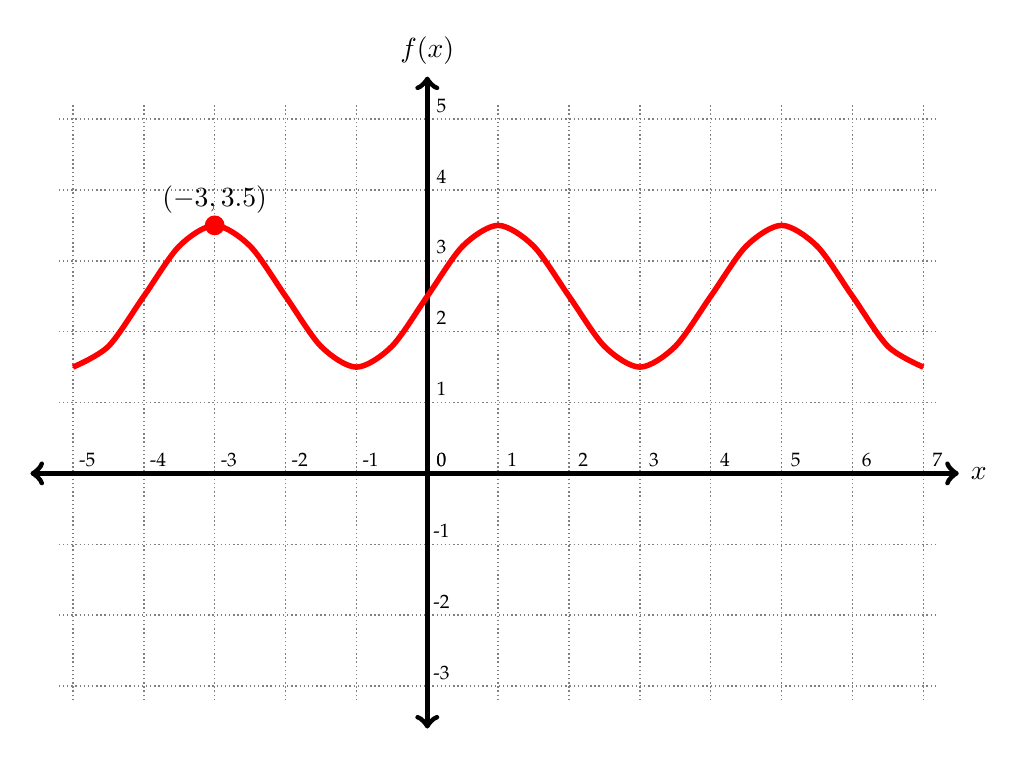
\begin{tikzpicture}[auto,scale=.9, line width=2pt]

\draw [line width=.5pt,densely dotted,gray] (-5.2,-3.2) grid (7.2,5.2);
\foreach \x in {-5,-4,...,7} \draw (\x+.2,.19) node {\scriptsize \x};
\foreach \y in {-3,-2,...,5} \draw (.2,\y+.19) node {\scriptsize \y};
\draw [<->] (-5.6,0) -- (7.5,0) node[right] {$x$};
\draw [<->] (0,-3.6) -- (0,5.6) node[above] {$f(x)$};

\draw[red,smooth] plot[domain=-5:7] (\x,{sin(90*\x) + 2.5}) ;

\draw[red,fill=red] (-3,3.5) circle (.1) node[above,black] {$(-3,3.5)$};

\end{tikzpicture}
\end{center}

%Filling and patterns

\begin{center}
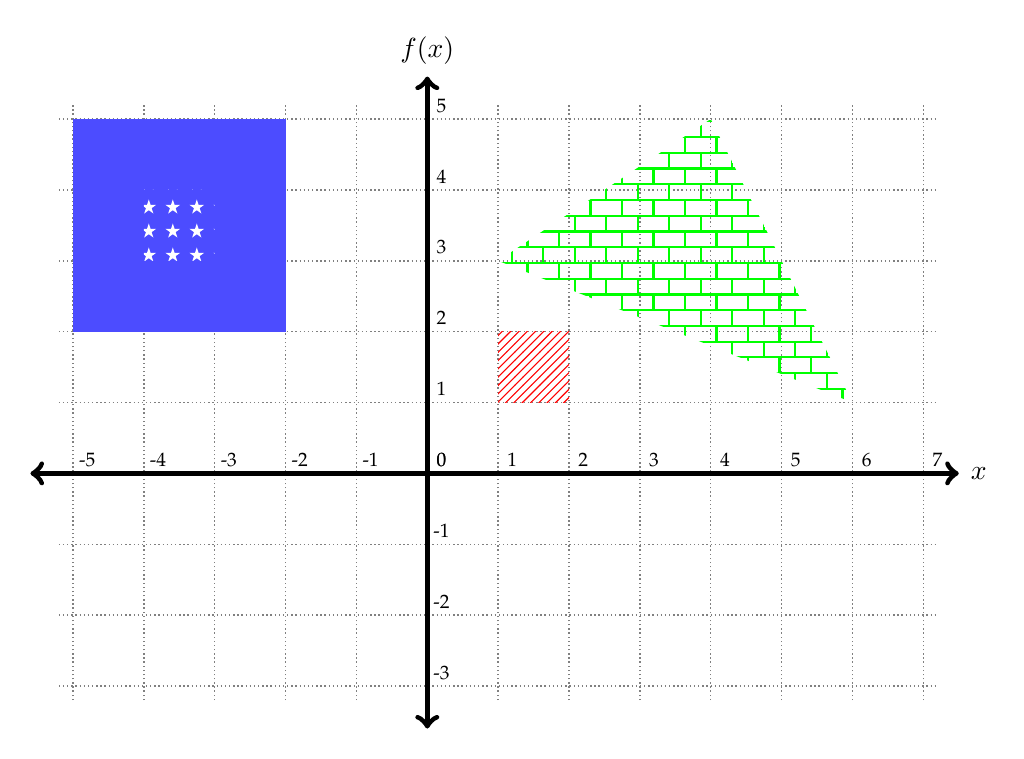
\begin{tikzpicture}[auto,scale=.9, line width=2pt]

\draw [line width=.5pt,densely dotted,gray] (-5.2,-3.2) grid (7.2,5.2);
\foreach \x in {-5,-4,...,7} \draw (\x+.2,.19) node {\scriptsize \x};
\foreach \y in {-3,-2,...,5} \draw (.2,\y+.19) node {\scriptsize \y};
\draw [<->] (-5.6,0) -- (7.5,0) node[right] {$x$};
\draw [<->] (0,-3.6) -- (0,5.6) node[above] {$f(x)$};

\fill[blue!70] (-5,2) -- (-2,2) -- (-2,5) -- (-5,5);
\fill[pattern color=white,pattern = fivepointed stars] (-4,3) -- (-3,3) -- (-3,4) -- (-4,4);

\fill[pattern color=red,pattern=north east lines] (1,1) -- (2,1) -- (2,2) -- (1,2);
\fill[pattern color = green,pattern=bricks] (1,3) -- (6,1) -- (4,5);

\end{tikzpicture}
\end{center}

\end{document}